\documentclass[11pt,]{article}
\usepackage[left=1in,top=1in,right=1in,bottom=1in]{geometry}
\newcommand*{\authorfont}{\fontfamily{phv}\selectfont}
\usepackage[]{mathpazo}


  \usepackage[T1]{fontenc}
  \usepackage[utf8]{inputenc}



\usepackage{abstract}
\renewcommand{\abstractname}{}    % clear the title
\renewcommand{\absnamepos}{empty} % originally center

\renewenvironment{abstract}
 {{%
    \setlength{\leftmargin}{0mm}
    \setlength{\rightmargin}{\leftmargin}%
  }%
  \relax}
 {\endlist}

\makeatletter
\def\@maketitle{%
  \newpage
%  \null
%  \vskip 2em%
%  \begin{center}%
  \let \footnote \thanks
    {\fontsize{18}{20}\selectfont\raggedright  \setlength{\parindent}{0pt} \@title \par}%
}
%\fi
\makeatother




\setcounter{secnumdepth}{0}

\usepackage{color}
\usepackage{fancyvrb}
\newcommand{\VerbBar}{|}
\newcommand{\VERB}{\Verb[commandchars=\\\{\}]}
\DefineVerbatimEnvironment{Highlighting}{Verbatim}{commandchars=\\\{\}}
% Add ',fontsize=\small' for more characters per line
\usepackage{framed}
\definecolor{shadecolor}{RGB}{248,248,248}
\newenvironment{Shaded}{\begin{snugshade}}{\end{snugshade}}
\newcommand{\KeywordTok}[1]{\textcolor[rgb]{0.13,0.29,0.53}{\textbf{#1}}}
\newcommand{\DataTypeTok}[1]{\textcolor[rgb]{0.13,0.29,0.53}{#1}}
\newcommand{\DecValTok}[1]{\textcolor[rgb]{0.00,0.00,0.81}{#1}}
\newcommand{\BaseNTok}[1]{\textcolor[rgb]{0.00,0.00,0.81}{#1}}
\newcommand{\FloatTok}[1]{\textcolor[rgb]{0.00,0.00,0.81}{#1}}
\newcommand{\ConstantTok}[1]{\textcolor[rgb]{0.00,0.00,0.00}{#1}}
\newcommand{\CharTok}[1]{\textcolor[rgb]{0.31,0.60,0.02}{#1}}
\newcommand{\SpecialCharTok}[1]{\textcolor[rgb]{0.00,0.00,0.00}{#1}}
\newcommand{\StringTok}[1]{\textcolor[rgb]{0.31,0.60,0.02}{#1}}
\newcommand{\VerbatimStringTok}[1]{\textcolor[rgb]{0.31,0.60,0.02}{#1}}
\newcommand{\SpecialStringTok}[1]{\textcolor[rgb]{0.31,0.60,0.02}{#1}}
\newcommand{\ImportTok}[1]{#1}
\newcommand{\CommentTok}[1]{\textcolor[rgb]{0.56,0.35,0.01}{\textit{#1}}}
\newcommand{\DocumentationTok}[1]{\textcolor[rgb]{0.56,0.35,0.01}{\textbf{\textit{#1}}}}
\newcommand{\AnnotationTok}[1]{\textcolor[rgb]{0.56,0.35,0.01}{\textbf{\textit{#1}}}}
\newcommand{\CommentVarTok}[1]{\textcolor[rgb]{0.56,0.35,0.01}{\textbf{\textit{#1}}}}
\newcommand{\OtherTok}[1]{\textcolor[rgb]{0.56,0.35,0.01}{#1}}
\newcommand{\FunctionTok}[1]{\textcolor[rgb]{0.00,0.00,0.00}{#1}}
\newcommand{\VariableTok}[1]{\textcolor[rgb]{0.00,0.00,0.00}{#1}}
\newcommand{\ControlFlowTok}[1]{\textcolor[rgb]{0.13,0.29,0.53}{\textbf{#1}}}
\newcommand{\OperatorTok}[1]{\textcolor[rgb]{0.81,0.36,0.00}{\textbf{#1}}}
\newcommand{\BuiltInTok}[1]{#1}
\newcommand{\ExtensionTok}[1]{#1}
\newcommand{\PreprocessorTok}[1]{\textcolor[rgb]{0.56,0.35,0.01}{\textit{#1}}}
\newcommand{\AttributeTok}[1]{\textcolor[rgb]{0.77,0.63,0.00}{#1}}
\newcommand{\RegionMarkerTok}[1]{#1}
\newcommand{\InformationTok}[1]{\textcolor[rgb]{0.56,0.35,0.01}{\textbf{\textit{#1}}}}
\newcommand{\WarningTok}[1]{\textcolor[rgb]{0.56,0.35,0.01}{\textbf{\textit{#1}}}}
\newcommand{\AlertTok}[1]{\textcolor[rgb]{0.94,0.16,0.16}{#1}}
\newcommand{\ErrorTok}[1]{\textcolor[rgb]{0.64,0.00,0.00}{\textbf{#1}}}
\newcommand{\NormalTok}[1]{#1}

\usepackage{graphicx,grffile}
\makeatletter
\def\maxwidth{\ifdim\Gin@nat@width>\linewidth\linewidth\else\Gin@nat@width\fi}
\def\maxheight{\ifdim\Gin@nat@height>\textheight\textheight\else\Gin@nat@height\fi}
\makeatother
% Scale images if necessary, so that they will not overflow the page
% margins by default, and it is still possible to overwrite the defaults
% using explicit options in \includegraphics[width, height, ...]{}
\setkeys{Gin}{width=\maxwidth,height=\maxheight,keepaspectratio}

\title{S02 - Distribución Gaussiana Multivariada  }



\author{\Large Juan Carlos Martinez-Ovando\vspace{0.05in} \newline\normalsize\emph{ITAM}  }


\date{}

\usepackage{titlesec}

\titleformat*{\section}{\normalsize\bfseries}
\titleformat*{\subsection}{\normalsize\itshape}
\titleformat*{\subsubsection}{\normalsize\itshape}
\titleformat*{\paragraph}{\normalsize\itshape}
\titleformat*{\subparagraph}{\normalsize\itshape}


\usepackage{natbib}
\bibliographystyle{plainnat}
\usepackage[strings]{underscore} % protect underscores in most circumstances



\newtheorem{hypothesis}{Hypothesis}
\usepackage{setspace}

\makeatletter
\@ifpackageloaded{hyperref}{}{%
\ifxetex
  \PassOptionsToPackage{hyphens}{url}\usepackage[setpagesize=false, % page size defined by xetex
              unicode=false, % unicode breaks when used with xetex
              xetex]{hyperref}
\else
  \PassOptionsToPackage{hyphens}{url}\usepackage[unicode=true]{hyperref}
\fi
}

\@ifpackageloaded{color}{
    \PassOptionsToPackage{usenames,dvipsnames}{color}
}{%
    \usepackage[usenames,dvipsnames]{color}
}
\makeatother
\hypersetup{breaklinks=true,
            bookmarks=true,
            pdfauthor={Juan Carlos Martinez-Ovando (ITAM)},
             pdfkeywords = {Graphical models, text analytics, contingency tables.},  
            pdftitle={S02 - Distribución Gaussiana Multivariada},
            colorlinks=true,
            citecolor=blue,
            urlcolor=blue,
            linkcolor=magenta,
            pdfborder={0 0 0}}
\urlstyle{same}  % don't use monospace font for urls

% set default figure placement to htbp
\makeatletter
\def\fps@figure{htbp}
\makeatother



% add tightlist ----------
\providecommand{\tightlist}{%
\setlength{\itemsep}{0pt}\setlength{\parskip}{0pt}}

\begin{document}
	
% \pagenumbering{arabic}% resets `page` counter to 1 
%
% \maketitle

{% \usefont{T1}{pnc}{m}{n}
\setlength{\parindent}{0pt}
\thispagestyle{plain}
{\fontsize{18}{20}\selectfont\raggedright 
\maketitle  % title \par  

}

{
   \vskip 13.5pt\relax \normalsize\fontsize{11}{12} 
\textbf{\authorfont Juan Carlos Martinez-Ovando} \hskip 15pt \emph{\small ITAM}   

}

}






\vskip 6.5pt


\noindent  \subsection{Paquetes}\label{paquetes}

\subsubsection{\texorpdfstring{\emph{Loading}}{Loading}}\label{loading}

Cargamos los paquetes que usaremos en estas ilustraciones.

\begin{Shaded}
\begin{Highlighting}[]
\ControlFlowTok{if}\NormalTok{ (}\KeywordTok{require}\NormalTok{(}\StringTok{"mvtnorm"}\NormalTok{) }\OperatorTok{==}\StringTok{ }\OtherTok{FALSE}\NormalTok{)\{}
  \KeywordTok{install.packages}\NormalTok{(}\StringTok{"mvtnorm"}\NormalTok{)}
\NormalTok{\}}
\end{Highlighting}
\end{Shaded}

\begin{verbatim}
## Loading required package: mvtnorm
\end{verbatim}

\begin{Shaded}
\begin{Highlighting}[]
\ControlFlowTok{if}\NormalTok{ (}\KeywordTok{require}\NormalTok{(}\StringTok{"MASS"}\NormalTok{) }\OperatorTok{==}\StringTok{ }\OtherTok{FALSE}\NormalTok{)\{}
  \KeywordTok{install.packages}\NormalTok{(}\StringTok{"mvtnorm"}\NormalTok{)}
\NormalTok{\}}
\end{Highlighting}
\end{Shaded}

\begin{verbatim}
## Loading required package: MASS
\end{verbatim}

\begin{Shaded}
\begin{Highlighting}[]
\KeywordTok{library}\NormalTok{(}\StringTok{"mvtnorm"}\NormalTok{,}\StringTok{"MASS"}\NormalTok{)}
\end{Highlighting}
\end{Shaded}

\section{Parte 1 - Teoria}\label{parte-1---teoria}

\subsection{Definicion}\label{definicion}

\subsubsection{\texorpdfstring{Caso Univariado
(\(p=1\))}{Caso Univariado (p=1)}}\label{caso-univariado-p1}

Iniciamos con la distribucion gaussiana unidimensional, acompanada por
una funcion de densidad de probabilidad,

\[
f(x|\mu,\sigma^2)
= 
(2\pi)^{-1/2} \sigma^{-1} \exp\left\{-(1/2\sigma^2) (x-\mu)^2\right\}
\] con soporte en \(\Re\) para \(x\).

\begin{itemize}
\tightlist
\item
  El espacio parametral para (\(\mu\),\(\sigma^2\)) es
  \$\Re \times \Re\_\{+\} \$.
\end{itemize}

\subsection{Definicion}\label{definicion-1}

\subsubsection{\texorpdfstring{Caso mulvivariado
(\(p<\infty\))}{Caso mulvivariado (p\textless{}\textbackslash{}infty)}}\label{caso-mulvivariado-pinfty}

El caso multivariado es una extension del univariado para
\(\boldsymbol{x}=(x_1,\ldots,x_p)\), pero que toma en cuenta las
interacciones entre las \(x_i\)s. Esta tiene una funcion de densidad
conjunta dada por,

\[
f(\boldsymbol{x}|\boldsymbol{\mu},\boldsymbol{\Sigma})
= 
(2\pi)^{-p/2} \det(\boldsymbol{\Sigma})^{-1/2} \exp\left\{-\frac{1}{2} (\boldsymbol{x}-\boldsymbol{\mu})'\boldsymbol{\Sigma}^{-1}(\boldsymbol{x}-\boldsymbol{\mu})\right\},
\] con soporte en \(\Re^{p}\) para \(\boldsymbol{x}\).

\begin{itemize}
\item
  El espacio parametral para \((\boldsymbol{\mu},\boldsymbol{\Sigma})\)
  es \(\Re^p \times \mathcal{M}_p\), donde \(\mathcal{M}_p\) denota el
  espacio de todas las matrices de dimension \(p \times p\) positivo
  definidas y simetricas.
\item
  Se denota como
  \(\boldsymbol{X} \sim N(\boldsymbol{x}|\boldsymbol{\mu},\boldsymbol{\Sigma})\).
\item
  El numero de parametros ``independientes'' en \(\boldsymbol{\mu}\) es
  igual a \(p\), mientras que el numero de parametros independientes en
  \(\boldsymbol{\Sigma}\) es igual a \(p(p+1)/2\).
\end{itemize}

\subsection{Propiedades}\label{propiedades}

\subsubsection{Propiedades basicas}\label{propiedades-basicas}

Si
\(\boldsymbol{X} \sim N(\boldsymbol{x}|\boldsymbol{\mu},\boldsymbol{\Sigma})\)
entonces,

\textbf{P1.} Cualquier combinacion lineal de \(\boldsymbol{X}\) es
gaussiana multivariada, i.e.~para todo \(A\) matriz de dimension
\(q\times p\) y \(c\) vector de dimension \(q \times 1\) se tiene que \[
\boldsymbol{Y}\sim N(\boldsymbol{y}|\boldsymbol{\mu}_y,\boldsymbol{\Sigma}_y),
\] con soporte para \(\boldsymbol{y}\) en \(\Re^{q}\), tal que

\[
\boldsymbol{\mu}_y = A\boldsymbol{\mu} + c,
\] y \[
\boldsymbol{\Sigma}_y = A\boldsymbol{\Sigma}A'.
\]

\subsection{Propiedades}\label{propiedades-1}

\subsubsection{Propiedades basicas}\label{propiedades-basicas-1}

Si
\(\boldsymbol{X} \sim N(\boldsymbol{x}|\boldsymbol{\mu},\boldsymbol{\Sigma})\)
entonces,

\textbf{P2.} Cualquier subconjunto de \(\boldsymbol{X}\) tiene una
distribucion gaussiana multivariada, i.e.~si
\(\boldsymbol{X}_{s}=(X_{s(1)},\ldots,X_{s(q)})\) (con \(q<p\)) es un
subconjuno de \(\boldsymbol{X}\) para un subconjunto de indices
\(\{s(1),\ldots,s(q)\}\) de \(\{1,\ldots,p\}\), entonces

\[
\boldsymbol{X}_{s} 
\sim
N(\boldsymbol{x}_{s}|\boldsymbol{\mu}_{s} ,\boldsymbol{\Sigma}_{s}),
\] donde \[
\boldsymbol{\mu}_s=(\mu_{s(1)},\ldots,\mu_{s(q)}),
\] y \[
\boldsymbol{\Sigma}_s=\left(\sigma_{s(i)s(j)}\right)_{i,j=1}^{q}.
\]

\subsection{Propiedades}\label{propiedades-2}

\subsubsection{Propiedades basicas}\label{propiedades-basicas-2}

Si
\(\boldsymbol{X} \sim N(\boldsymbol{x}|\boldsymbol{\mu},\boldsymbol{\Sigma})\)
entonces,

\textbf{P3.} Si un subconjunto de \(\boldsymbol{X}\) no esta
correlacionado, entonces las variables de ese conjunto son
\emph{estocasticamente independientes}, i.e.

\begin{itemize}
\tightlist
\item
  Si \((X_i,X_j)\) son un subconjunto de \(\boldsymbol{X}\) (con
  \(i,j<p\)), tales que \[\sigma_{i,j}=0,\] entonces \(X_i\) y \(X_j\)
  son independientes estocasticamente con, \[
  f(x_i,x_j|\mu_i,\mu_j,\sigma_{ii},\sigma_{jj},\sigma_{ij}) = N(x_i|\mu_i,\sigma_{ii})\times N(x_j|\mu_j,\sigma_{jj}).
  \]
\end{itemize}

\subsection{Propiedades}\label{propiedades-3}

\subsubsection{Propiedades basicas}\label{propiedades-basicas-3}

Si
\(\boldsymbol{X} \sim N(\boldsymbol{x}|\boldsymbol{\mu},\boldsymbol{\Sigma})\)
entonces,

\textbf{P4.} Si un \(A\) y \(B\) son dos matrices de dimension
(\(q\times p\)) tales que \[
A\boldsymbol{\Sigma}B' = \boldsymbol{0},
\] de dimension \(q\times q\), entonces

\begin{itemize}
\tightlist
\item
  las variables \[
  \boldsymbol{Y}_A = A\boldsymbol{X} \ \text{ y } \
  \boldsymbol{Y}_B = B\boldsymbol{X},
  \] son \emph{estocasticamente independientes}.
\end{itemize}

\subsection{Condicionamiento}\label{condicionamiento}

\subsubsection{Distribuciones
condicionales}\label{distribuciones-condicionales}

Supongamos que \(\boldsymbol{X}=(\boldsymbol{X}_1,\boldsymbol{X}_2)\),
donde ambos componentes son de dimension \(p_1\) y \(p_2\)
respectivamente (\(p=p_1+p_2\)).

\begin{itemize}
\item
  Lo anterior se conoce como una particion de dos componentes de
  \(\boldsymbol{X}\).
\item
  Los parametros del modelo tambien estan particionados, i.e. \[
  \boldsymbol{\mu} = (\boldsymbol{\mu}_1,\boldsymbol{\mu}_2).
  \]
\end{itemize}

\[
\boldsymbol{\Sigma} = 
\left(
\begin{array}{cc}
\boldsymbol{\Sigma}_{11} & \boldsymbol{\Sigma}_{12} \\
\boldsymbol{\Sigma}_{21} & \boldsymbol{\Sigma}_{22}
\end{array}
\right).
\]

\begin{itemize}
\tightlist
\item
  La \emph{distribucion marginal} de \(\boldsymbol{X}_i\) (\(i=1,2\) )
  es \[
  \boldsymbol{X}_i \sim N(\boldsymbol{x}_i|\boldsymbol{\mu}_i,\boldsymbol{\Sigma}_i).
  \]
\end{itemize}

\subsection{Condicionamiento}\label{condicionamiento-1}

\subsubsection{\texorpdfstring{Distribucion condicional
\(\boldsymbol{X}_2|\boldsymbol{X}_1=\boldsymbol{x}_1\)}{Distribucion condicional \textbackslash{}boldsymbol\{X\}\_2\textbar{}\textbackslash{}boldsymbol\{X\}\_1=\textbackslash{}boldsymbol\{x\}\_1}}\label{distribucion-condicional-boldsymbolx_2boldsymbolx_1boldsymbolx_1}

\textbf{P5.} La distribucion condicional de \(\boldsymbol{X}_2\) dado
\(\boldsymbol{X}_1=\boldsymbol{x}_1\) es gaussiana multivariada, con \[
\boldsymbol{X}_2|\boldsymbol{X}_1=\boldsymbol{x}_1
\sim
N\left(\boldsymbol{x}_2|\boldsymbol{\mu}_{2|1},\boldsymbol{\Sigma}_{2|1}\right),
\] donde \[
\boldsymbol{\mu}_{2|1} = \boldsymbol{\mu}_2 + \boldsymbol{\Sigma}_{21}\boldsymbol{\Sigma}_{11}^{-1}(\boldsymbol{x}_1-\boldsymbol{\mu}_1),
\] y \[
\boldsymbol{\Sigma}_{2|1} = \boldsymbol{\Sigma}_{22} - \boldsymbol{\Sigma}_{21}\boldsymbol{\Sigma}_{11}^{-1}\boldsymbol{\Sigma}_{12}.
\]

\begin{itemize}
\tightlist
\item
  Esta propiedad es simetrica, en el sentido que la distribucion
  condicional de \(\boldsymbol{X}_1|\boldsymbol{X}_2=\boldsymbol{x}_2\)
  es analoga.
\end{itemize}

\subsection{Descomposicion}\label{descomposicion}

\subsubsection{Estructura espectral}\label{estructura-espectral}

\textbf{Definicion.-} Una matrix \(P\) de dimension \(p\times p\) es
\emph{ortogonal} si \(P P' = P' P=I\).

\textbf{TEOREMA:} Una matrix \(A\) simetrica de dimension \(p\times p\)
puede reexpresarse como \[A=P \Lambda P',\] donde

\begin{itemize}
\item
  \(\Lambda = diag\{\lambda_1,\ldots,\lambda_p\}\) de
  \emph{eigenvalores}
\item
  \(P\) es una matriz ortogonal de eigenvectores columna.
\end{itemize}

\textbf{INTUICION}

\begin{itemize}
\item
  La matriz de \emph{eigenvalores} representa \emph{rotaciones} de
  coordenadas.
\item
  La matriz de \emph{eigenvalores} representan \emph{contracciones} o
  \emph{expansiones} de coordenadas.
\end{itemize}

\subsection{Descomposicion}\label{descomposicion-1}

\subsubsection{Acerca de determinantes}\label{acerca-de-determinantes}

\textbf{PROPIEDAD.-} Bajo la descomposicion espectral de
\(\boldsymbol{\Sigma}\) se sigue
\[\det(\boldsymbol{\Sigma})=\prod_{j=1}^{p}\lambda_j.\]

\textbf{INTUICION}

\begin{itemize}
\item
  Los \emph{eigenvalores} de \(\boldsymbol{\Sigma}\) nos indican el
  grado de variabilidad de cada dimension (por separado)
\item
  Los \(\lambda_j\)s nos indican que tan expandida/contraida es la
  distribucion en esta dimension
\item
  El factor \(\det(\boldsymbol{\Sigma})\) puede verse como un factor de
  expansion/contraccion de la distribucion gaussiana conjunta
\end{itemize}

\subsection{Visualizacion}\label{visualizacion}

\subsubsection{Contornos}\label{contornos}

La grafica de \textbf{contornos} nos permiten visualizar distribuciones
gaussianas de dos dimensiones (i.e.~es una representacion de graficas en
3D).

Los \emph{contronos} se obtienen como \emph{rebanadas} de la densidad
conjunta en 2D.

Las lineas representan la coleccion de valores de \(\boldsymbol{x}\) que
comparten el mismo nivel de \(N(\boldsymbol{x}|\mu,\Sigma)\).

\textbf{Propiedad.-} Los contornos se definen en terminos de \(\Lambda\)
y \(P\) como \textbf{elipsoides}
\[||\boldsymbol{\Sigma}^{-1/2}(\boldsymbol{x}-\boldsymbol{\mu})||=c^{2},\]
siendo centradas en \(\boldsymbol{\mu}\) y con ejes en la direccion
\(\sqrt{\lambda_j p_j}\).

\subsection{Visualizacion}\label{visualizacion-1}

\subsubsection{Contornos}\label{contornos-1}

Visualizacion de datos por contornos con \textbf{dependencia nula}.

\begin{Shaded}
\begin{Highlighting}[]
\NormalTok{x.points <-}\StringTok{ }\KeywordTok{seq}\NormalTok{(}\OperatorTok{-}\DecValTok{3}\NormalTok{,}\DecValTok{3}\NormalTok{,}\DataTypeTok{length.out=}\DecValTok{100}\NormalTok{)}
\NormalTok{y.points <-}\StringTok{ }\NormalTok{x.points}
\NormalTok{z <-}\StringTok{ }\KeywordTok{matrix}\NormalTok{(}\DecValTok{0}\NormalTok{,}\DataTypeTok{nrow=}\DecValTok{100}\NormalTok{,}\DataTypeTok{ncol=}\DecValTok{100}\NormalTok{)}
\NormalTok{mu <-}\StringTok{ }\KeywordTok{c}\NormalTok{(}\DecValTok{0}\NormalTok{,}\DecValTok{0}\NormalTok{)}
\NormalTok{sigma <-}\StringTok{ }\KeywordTok{matrix}\NormalTok{(}\KeywordTok{c}\NormalTok{(}\DecValTok{2}\NormalTok{,}\DecValTok{0}\NormalTok{,}\DecValTok{0}\NormalTok{,}\DecValTok{1}\NormalTok{),}\DataTypeTok{nrow=}\DecValTok{2}\NormalTok{)}
\ControlFlowTok{for}\NormalTok{(i }\ControlFlowTok{in} \DecValTok{1}\OperatorTok{:}\DecValTok{100}\NormalTok{)\{}
  \ControlFlowTok{for}\NormalTok{(j }\ControlFlowTok{in} \DecValTok{1}\OperatorTok{:}\DecValTok{100}\NormalTok{)\{}
\NormalTok{    z[i,j] <-}\StringTok{ }\KeywordTok{dmvnorm}\NormalTok{(}\KeywordTok{c}\NormalTok{(x.points[i],y.points[j]),}
                      \DataTypeTok{mean=}\NormalTok{mu,}\DataTypeTok{sigma=}\NormalTok{sigma)}
\NormalTok{    \}}
\NormalTok{\}}
\KeywordTok{png}\NormalTok{(}\StringTok{"C:/Users/jcmo/Google Drive/Material.Cursos/EST46114/Sesiones/est46114/figuras/contour_nula.png"}\NormalTok{, }\DecValTok{490}\NormalTok{, }\DecValTok{490}\NormalTok{)}
\KeywordTok{contour}\NormalTok{(x.points,y.points,z)}
\KeywordTok{dev.off}\NormalTok{()}
\end{Highlighting}
\end{Shaded}

\begin{verbatim}
## pdf 
##   2
\end{verbatim}

\subsection{Visualizacion}\label{visualizacion-2}

\begin{figure}
\centering
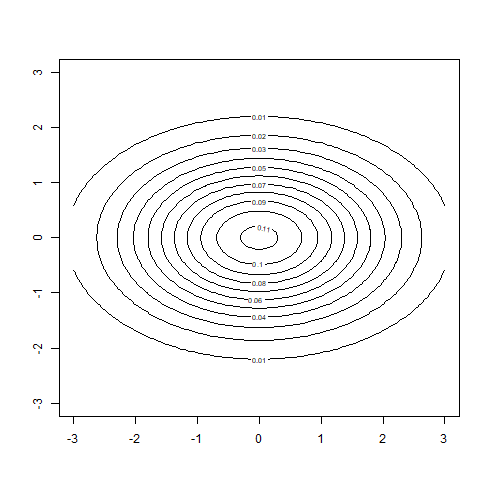
\includegraphics{C:/Users/jcmo/Google\%20Drive/Material.Cursos/EST46114/Sesiones/est46114/figuras/contour_nula.png}
\caption{Contornos de distribucion gausiana.}
\end{figure}

\subsection{Visualizacion}\label{visualizacion-3}

\subsubsection{Contornos}\label{contornos-2}

Visualizacion de datos por contornos con \textbf{dependencia positiva.}

\begin{Shaded}
\begin{Highlighting}[]
\NormalTok{x.points <-}\StringTok{ }\KeywordTok{seq}\NormalTok{(}\OperatorTok{-}\DecValTok{3}\NormalTok{,}\DecValTok{3}\NormalTok{,}\DataTypeTok{length.out=}\DecValTok{100}\NormalTok{)}
\NormalTok{y.points <-}\StringTok{ }\NormalTok{x.points}
\NormalTok{z <-}\StringTok{ }\KeywordTok{matrix}\NormalTok{(}\DecValTok{0}\NormalTok{,}\DataTypeTok{nrow=}\DecValTok{100}\NormalTok{,}\DataTypeTok{ncol=}\DecValTok{100}\NormalTok{)}
\NormalTok{mu <-}\StringTok{ }\KeywordTok{c}\NormalTok{(}\DecValTok{0}\NormalTok{,}\DecValTok{0}\NormalTok{)}
\NormalTok{sigma <-}\StringTok{ }\KeywordTok{matrix}\NormalTok{(}\KeywordTok{c}\NormalTok{(}\DecValTok{2}\NormalTok{,}\DecValTok{1}\NormalTok{,}\DecValTok{1}\NormalTok{,}\DecValTok{1}\NormalTok{),}\DataTypeTok{nrow=}\DecValTok{2}\NormalTok{)}
\ControlFlowTok{for}\NormalTok{(i }\ControlFlowTok{in} \DecValTok{1}\OperatorTok{:}\DecValTok{100}\NormalTok{)\{}
  \ControlFlowTok{for}\NormalTok{(j }\ControlFlowTok{in} \DecValTok{1}\OperatorTok{:}\DecValTok{100}\NormalTok{)\{}
\NormalTok{    z[i,j] <-}\StringTok{ }\KeywordTok{dmvnorm}\NormalTok{(}\KeywordTok{c}\NormalTok{(x.points[i],y.points[j]),}
                      \DataTypeTok{mean=}\NormalTok{mu,}\DataTypeTok{sigma=}\NormalTok{sigma)}
\NormalTok{    \}}
\NormalTok{\}}
\KeywordTok{png}\NormalTok{(}\StringTok{"C:/Users/jcmo/Google Drive/Material.Cursos/EST46114/Sesiones/est46114/figuras/contour_positiva.png"}\NormalTok{, }\DecValTok{490}\NormalTok{, }\DecValTok{490}\NormalTok{)}
\KeywordTok{contour}\NormalTok{(x.points,y.points,z)}
\KeywordTok{dev.off}\NormalTok{()}
\end{Highlighting}
\end{Shaded}

\begin{verbatim}
## pdf 
##   2
\end{verbatim}

\subsection{Visualizacion}\label{visualizacion-4}

\begin{figure}
\centering
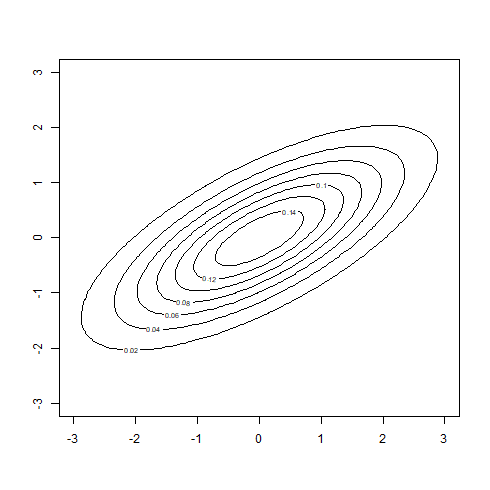
\includegraphics{C:/Users/jcmo/Google\%20Drive/Material.Cursos/EST46114/Sesiones/est46114/figuras/contour_positiva.png}
\caption{Contornos de distribucion gausiana con covarianza positiva}
\end{figure}

\subsection{Visualizacion}\label{visualizacion-5}

\subsubsection{Contornos}\label{contornos-3}

Visualizacion de datos por contornos con \textbf{dependencia negativa.}

\begin{Shaded}
\begin{Highlighting}[]
\NormalTok{x.points <-}\StringTok{ }\KeywordTok{seq}\NormalTok{(}\OperatorTok{-}\DecValTok{3}\NormalTok{,}\DecValTok{3}\NormalTok{,}\DataTypeTok{length.out=}\DecValTok{100}\NormalTok{)}
\NormalTok{y.points <-}\StringTok{ }\NormalTok{x.points}
\NormalTok{z <-}\StringTok{ }\KeywordTok{matrix}\NormalTok{(}\DecValTok{0}\NormalTok{,}\DataTypeTok{nrow=}\DecValTok{100}\NormalTok{,}\DataTypeTok{ncol=}\DecValTok{100}\NormalTok{)}
\NormalTok{mu <-}\StringTok{ }\KeywordTok{c}\NormalTok{(}\DecValTok{0}\NormalTok{,}\DecValTok{0}\NormalTok{)}
\NormalTok{sigma <-}\StringTok{ }\KeywordTok{matrix}\NormalTok{(}\KeywordTok{c}\NormalTok{(}\DecValTok{2}\NormalTok{,}\OperatorTok{-}\DecValTok{1}\NormalTok{,}\OperatorTok{-}\DecValTok{1}\NormalTok{,}\DecValTok{1}\NormalTok{),}\DataTypeTok{nrow=}\DecValTok{2}\NormalTok{)}
\ControlFlowTok{for}\NormalTok{(i }\ControlFlowTok{in} \DecValTok{1}\OperatorTok{:}\DecValTok{100}\NormalTok{)\{}
  \ControlFlowTok{for}\NormalTok{(j }\ControlFlowTok{in} \DecValTok{1}\OperatorTok{:}\DecValTok{100}\NormalTok{)\{}
\NormalTok{    z[i,j] <-}\StringTok{ }\KeywordTok{dmvnorm}\NormalTok{(}\KeywordTok{c}\NormalTok{(x.points[i],y.points[j]),}
                      \DataTypeTok{mean=}\NormalTok{mu,}\DataTypeTok{sigma=}\NormalTok{sigma)}
\NormalTok{    \}}
\NormalTok{\}}
\KeywordTok{png}\NormalTok{(}\StringTok{"C:/Users/jcmo/Google Drive/Material.Cursos/EST46114/Sesiones/est46114/figuras/contour_negativa.png"}\NormalTok{, }\DecValTok{490}\NormalTok{, }\DecValTok{490}\NormalTok{)}
\KeywordTok{contour}\NormalTok{(x.points,y.points,z)}
\KeywordTok{dev.off}\NormalTok{()}
\end{Highlighting}
\end{Shaded}

\begin{verbatim}
## pdf 
##   2
\end{verbatim}

\subsection{Visualizacion}\label{visualizacion-6}

\begin{figure}
\centering
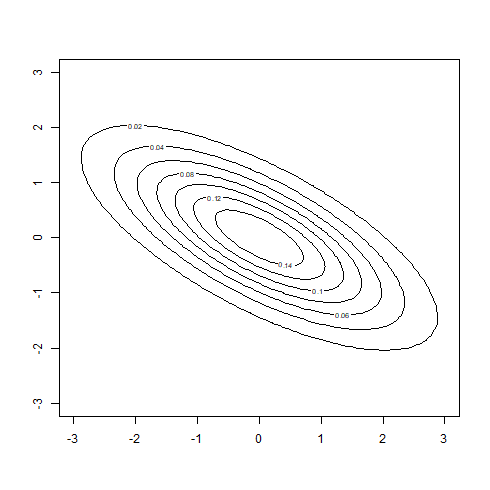
\includegraphics{C:/Users/jcmo/Google\%20Drive/Material.Cursos/EST46114/Sesiones/est46114/figuras/contour_negativa.png}
\caption{Contornos de distribucion gausiana con covarianza positiva}
\end{figure}

\section{Parte 2 - Practica}\label{parte-2---practica}

\subsection{Exploracion 1:1}\label{exploracion-11}

\begin{Shaded}
\begin{Highlighting}[]
\NormalTok{data01 <-}\StringTok{ }\KeywordTok{read.csv}\NormalTok{(}\DataTypeTok{file=}\StringTok{"C:/Users/jcmo/Google Drive/Material.Cursos/EST46114/Sesiones/est46114/datos/est46114_semana02.csv"}\NormalTok{,}\DataTypeTok{header=}\OtherTok{TRUE}\NormalTok{)}
\KeywordTok{summary}\NormalTok{(data01)}
\end{Highlighting}
\end{Shaded}

\begin{verbatim}
##        X1              X2       
##  Min.   :340.0   Min.   :240.0  
##  1st Qu.:470.0   1st Qu.:450.0  
##  Median :500.0   Median :500.0  
##  Mean   :499.3   Mean   :498.3  
##  3rd Qu.:530.0   3rd Qu.:550.0  
##  Max.   :640.0   Max.   :730.0
\end{verbatim}

\begin{Shaded}
\begin{Highlighting}[]
\NormalTok{X <-}\StringTok{ }\KeywordTok{cbind}\NormalTok{(data01}\OperatorTok{$}\NormalTok{X1,data01}\OperatorTok{$}\NormalTok{X2)}
\end{Highlighting}
\end{Shaded}

\subsection{Visualizacion}\label{visualizacion-7}

\subsubsection{Nubes}\label{nubes}

Scatter plot (nube de datos eliptica)

\begin{Shaded}
\begin{Highlighting}[]
\KeywordTok{plot}\NormalTok{(X)}
\end{Highlighting}
\end{Shaded}

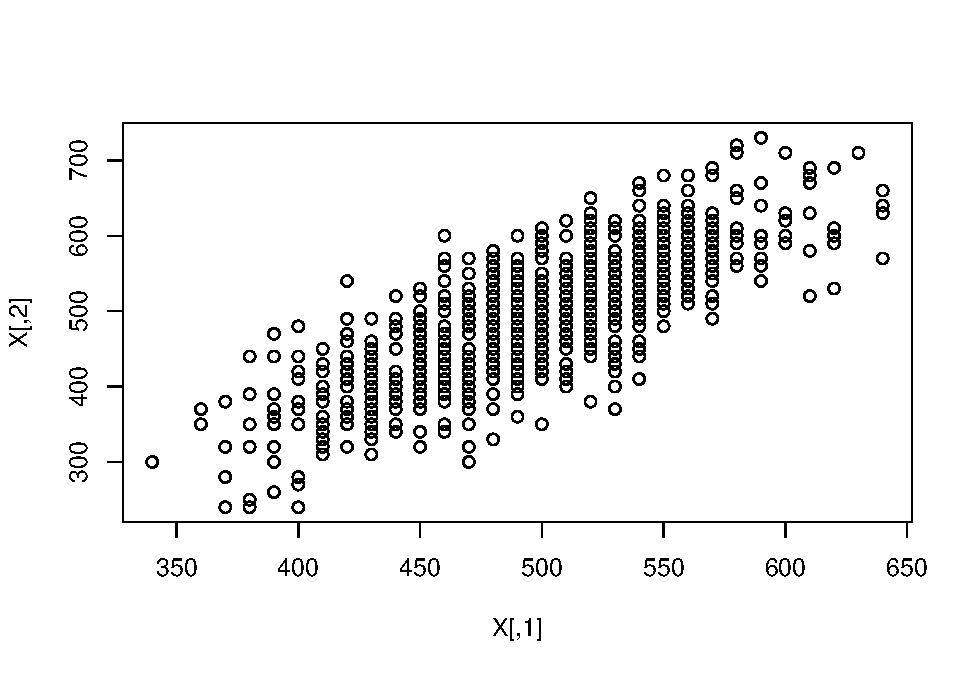
\includegraphics{est46114_s02_gaussianamultivariada_files/figure-latex/plot_nube-1.pdf}

\subsection{Verosimilitud}\label{verosimilitud}

La funcion de verosimilitud para \((\mu,\Sigma)\) condicional en un
conjunto de datos, \(\boldsymbol{x}_1,\ldots,\boldsymbol{x}_n\) se
calcula como la distribucion conjunta de los \(n\) datos, la cual toma
la forma \[
l(\mu,\Sigma|\boldsymbol{x}_1,\ldots,\boldsymbol{x}_n) = \prod_{i}N(\boldsymbol{x}_i|\mu,\Sigma) \\
\propto |\Sigma|^{-n/2}\exp\left\{-\frac{1}{2}\sum_{i}(x_i-\mu)'\Sigma^{-1}(x_i-\mu)\right\}\\
\propto |\Sigma|^{-n/2}\exp\left\{-\frac{1}{2}tr\left(\Sigma^{-1}(S+dd')\right)\right\},
\] donde \(d=\bar{x}-\mu\) y \(S\) es la matriz de covarianzas muestral.

\subsection{Verosimilitud}\label{verosimilitud-1}

\subsubsection{Computo}\label{computo}

La funcion de verosimilitud para \((\mu,\Sigma)\) condicional en un
conjunto de




\newpage
\singlespacing 
\end{document}
